\documentclass[english,xcolor=svgnames]{beamer}


\usepackage{mathptmx}
\usepackage[OT1]{fontenc}
% \usepackage[latin9]{inputenc}
\usepackage{amsmath}
\usepackage{amssymb}
\usepackage{amsthm}
\usepackage{mathrsfs}
\usepackage{amsfonts}
\usepackage{eurosym}
\usepackage{bm}

\usepackage{booktabs}
\usepackage{tabularx}
\usepackage{subcaption}
\usepackage[makeroom,thicklines]{cancel}

\usepackage{multirow}
\usepackage{rotating}
\usepackage{array}
\usepackage{float}



\makeatletter

 \newcommand\makebeamertitle{\frame{\maketitle}}%
 \AtBeginDocument{
   \let\origtableofcontents=\tableofcontents
 \def\tableofcontents{\@ifnextchar[{\origtableofcontents}{\gobbletableofcontents}}
   \def\gobbletableofcontents#1{\origtableofcontents}
 }
 
 \usetheme{Boadilla}
\setbeamertemplate{footline}[frame number]{}
\usefonttheme{structuresmallcapsserif}
\setbeamercolor{title}{fg=blue}
\setbeamercolor{frametitle}{fg=blue}
\setbeamercolor{caption name}{fg=blue}
\setbeamercovered{transparent}


\beamertemplatenavigationsymbolsempty

\usepackage{booktabs}
\usepackage{tabularx}
\renewcommand{\tabularxcolumn}[1]{>{\centering\arraybackslash}m{#1}}
%\newcolumntype{L}{>{\centering}X}
%\newcolumntype{H}{>{\lrbox0}c<{\endlrbox}@{}}

%\let\estinput=\input
%\newcommand{\estwide}[3]{
%          \vspace{.75ex}{
%               \begin{tabularx}
%               {\textwidth}{@{\hskip\tabcolsep\extracolsep\fill}l*{#2}{#3}}
%               \toprule
%               \estinput{#1}
%               \bottomrule
%               \addlinespace[.75ex]
%               \end{tabularx}
%               }
%          }
%
%		\newcommand{\figtext}[1]{
%		     %\vspace{-1.9ex}
%		     \captionsetup{justification=justified,font=footnotesize}
%		     \caption*{\hspace{6pt}\hangindent=1.5em #1}
%		     }
%		\newcommand{\fignote}[1]{\figtext{\emph{Note:~}~#1}}
%
\usepackage{collcell}
%\makeatother
% \newcolumntype{G}{>{\collectcell\@gobble}c<{\endcollectcell}@{}}
% \makeatother
% \def\eatcell#1\unskip{}
% \newcolumntype{E}{>{\eatcell}c@{}}
%\usepackage{tabulary}
%\usepackage{multirow}
%\usepackage{dcolumn}
%\usepackage{pdflscape}
%\usepackage{pdfpages}
% \usepackage{epsfig}
% \usepackage{epstopdf}
% \usepackage{eso-pic}
\usepackage{graphicx}
%\usepackage{arydshln}
\usepackage[compatibility=false,font={sc,rm,color=blue},justification=centering,labelformat=empty, textfont=Large, margin=2pt]{caption}
\captionsetup[figure]{belowskip=0pt}

\newcommand{\rot}[2]{\rule{1em}{0pt}%
\makebox[0cm][c]{\rotatebox{#1}{\ #2}}}

\usepackage{siunitx} %For aligning decimals
\sisetup{ detect-mode, 
          group-digits            = false ,
          input-signs             = ,
          input-symbols           = ()[]-+* ,
          input-open-uncertainty  = ,
          input-close-uncertainty = ,
          table-align-text-post   = false, 
          table-number-alignment = center
}
\selectcolormodel{cmyk}
\usepackage{color,soul}
\usepackage{colortbl}
\usepackage{tikz}
\usetikzlibrary{matrix,shapes,arrows,intersections,calc}
\usepackage{verbatim}
\setbeamercovered{invisible}
\setbeamercolor{math text displayed}{fg=blue}
\setbeamercolor{math text inlined}{fg=blue}

%\let\olditem\item
%\renewcommand{\item}{\setlength{\itemsep}{\fill}\olditem}
\AtBeginDocument{\setlength\belowdisplayskip{0pt}}


\usepackage[english]{babel}
\usepackage{booktabs}
\usepackage{tablefootnote}
\usepackage{calc,hhline,ifthen,lscape} 

%\usepackage{enumitem}
%\let\olditem\item
%\renewcommand{\item}{\setlength{\itemsep}{\fill}\olditem}

% new math commands
\newcommand{\E}{\mathbb{E}}

\newcommand{\sym}[1]{\rlap{$#1$}} %For sym in STATA tables

\setbeamertemplate{frametitle}[default][center]

% \makeglossaries
% 
% \usepackage{pgfpages}
% \pgfpagesuselayout{resize to}[a4paper, landscape, border shrink=5mm]
\usepackage[absolute,overlay]{textpos}

\usepackage{epstopdf}


%\setlength{\itemsep}{\fill}



% ===========================================================
% ===========================================================
% ===========================================================
% Improves spacing of itemize and enumerate environment

\makeatletter
\renewcommand{\itemize}[1][]{%
  \beamer@ifempty{#1}{}{\def\beamer@defaultospec{#1}}%
  \ifnum \@itemdepth >2\relax\@toodeep\else
    \advance\@itemdepth\@ne
    \beamer@computepref\@itemdepth% sets \beameritemnestingprefix
    \usebeamerfont{itemize/enumerate \beameritemnestingprefix body}%
    \usebeamercolor[fg]{itemize/enumerate \beameritemnestingprefix body}%
    \usebeamertemplate{itemize/enumerate \beameritemnestingprefix body begin}%
    \list
      {\usebeamertemplate{itemize \beameritemnestingprefix item}}
      {\def\makelabel##1{%
          {%
            \hss\llap{{%
                \usebeamerfont*{itemize \beameritemnestingprefix item}%
                \usebeamercolor[fg]{itemize \beameritemnestingprefix item}##1}}%
          }%
        }%
      }
  \fi%
  \setlength\itemsep{\fill}
    \ifnum \@itemdepth >1
        \vfill
    \fi%  
  \beamer@cramped%
  \raggedright%
  \beamer@firstlineitemizeunskip%
}

\def\enditemize{\ifhmode\unskip\fi\endlist%
  \usebeamertemplate{itemize/enumerate \beameritemnestingprefix body end}
  \ifnum \@itemdepth >1
        \vfil
  \fi%  
  }
\makeatother


\makeatletter
\def\enumerate{%
	\ifnum\@enumdepth>2\relax\@toodeep
	\else%
	\advance\@enumdepth\@ne%
	\edef\@enumctr{enum\romannumeral\the\@enumdepth}%
	\advance\@itemdepth\@ne%
	\fi%
	\beamer@computepref\@enumdepth% sets \beameritemnestingprefix
	\edef\beamer@enumtempl{enumerate \beameritemnestingprefix item}%
	\@ifnextchar[{\beamer@@enum@}{\beamer@enum@}}
\def\beamer@@enum@[{\@ifnextchar<{\beamer@enumdefault[}{\beamer@@@enum@[}}
\def\beamer@enumdefault[#1]{\def\beamer@defaultospec{#1}%
	\@ifnextchar[{\beamer@@@enum@}{\beamer@enum@}}
\def\beamer@@@enum@[#1]{% partly copied from enumerate.sty
	\@enLab{}\let\@enThe\@enQmark
	\@enloop#1\@enum@
	\ifx\@enThe\@enQmark\@warning{The counter will not be printed.%
		^^J\space\@spaces\@spaces\@spaces The label is: \the\@enLab}\fi
	\def\insertenumlabel{\the\@enLab}
	\def\beamer@enumtempl{enumerate mini template}%
	\expandafter\let\csname the\@enumctr\endcsname\@enThe
	\csname c@\@enumctr\endcsname7
	\expandafter\settowidth
	\csname leftmargin\romannumeral\@enumdepth\endcsname
	{\the\@enLab\hspace{\labelsep}}%
	\beamer@enum@}
\def\beamer@enum@{%
	\beamer@computepref\@itemdepth% sets \beameritemnestingprefix
	\usebeamerfont{itemize/enumerate \beameritemnestingprefix body}%
	\usebeamercolor[fg]{itemize/enumerate \beameritemnestingprefix body}%
	\usebeamertemplate{itemize/enumerate \beameritemnestingprefix body begin}%
	\expandafter
	\list
	{\usebeamertemplate{\beamer@enumtempl}}
	{\usecounter\@enumctr%
		\def\makelabel##1{{\hss\llap{{%
						\usebeamerfont*{enumerate \beameritemnestingprefix item}%
						\usebeamercolor[fg]{enumerate \beameritemnestingprefix item}##1}}}}}%
	\setlength\itemsep{\fill}
	\ifnum \@itemdepth >1
	\vfill
	\fi%  
	\beamer@cramped%
	\raggedright%
	\beamer@firstlineitemizeunskip%
}
\def\endenumerate{\ifhmode\unskip\fi\endlist%
	\usebeamertemplate{itemize/enumerate \beameritemnestingprefix body end}
	\ifnum \@itemdepth >1
	\vfil
	\fi%  
}
\makeatother

% ===========================================================
% ===========================================================
% ===========================================================


%\usepackage[colorlinks=true]{hyperref}

\hypersetup{colorlinks = true,linkcolor = blue, bookmarksopen=true, bookmarksopenlevel=1}

%\hypersetup{bookmarksopen=true, bookmarksopenlevel=1}



\begin{document}

\title{The Sequence Space}
\vspace{1cm}
\author[shortname]{
\begin{tabular}{cc}
Juan Herre\~{n}o & Johannes Wieland \\ 
\end{tabular}\\
}



\date{UCSD, Spring \the\year}

\setbeamertemplate{footline}{}
\makebeamertitle
\setbeamertemplate{footline}[frame number]{}

\addtocounter{framenumber}{-1}



%\begin{frame}
%\frametitle[alignment=center]{Reminders}
%\begin{enumerate}
%	\item First project draft due May 1.
%	\item Participation.
%\end{enumerate}
%\end{frame}


%%%%%%%%%%%%%%%%%%%%%%%%%%%%%%%%%%%%%%%%%%%%%%%%%%
\AtBeginSection[]{
\setbeamertemplate{footline}{}
  \frame<beamer>{ 

    \frametitle{Outline}   

    \tableofcontents[currentsection,hideallsubsections] 
  }
\setbeamertemplate{footline}[frame number]{}
\addtocounter{framenumber}{-1}
}

\AtBeginSubsection[]{
\setbeamertemplate{footline}{}
  \frame<beamer>{ 

    \frametitle{Outline}   

    \tableofcontents[currentsection,currentsubsection] 
  }
  \setbeamertemplate{footline}[frame number]{}
  \addtocounter{framenumber}{-1}
}



\setbeamertemplate{footline}{}
\begin{frame}
\frametitle{Outline}   
\tableofcontents[hideallsubsections] 
\end{frame}
\addtocounter{framenumber}{-1}
\setbeamertemplate{footline}[frame number]{}


%%%%%%%%%%%%%%%%%%%%%%%%%%%%%%%%%%%%%%%%%%%%%%%%%%
\section{Introduction}
%%%%%%%%%%%%%%%%%%%%%%%%%%%%%%%%%%%%%%%%%%%%%%%%%%


\begin{frame}
    \frametitle{Solving Models}
    \begin{itemize}
        \item Hard when there is rich heterogeneity.
        \item Infinitely dimensional state space from the distribution of agent's endogenous state variables---how to handle it?
        \item In macro, we are often interested what happens when aggregate shock X hits the economy (monetary, fiscal, etc).
        \item State space: must forecast infinite-dimensional distribution to estimate prices / quantities relevant to agents' problem.
        \item Sequence space: must find price / quantity sequences that solve market clearing conditions.
        \item[$\Rightarrow$] Sequence space is of dimension $T \times \text{number of variables}$, versus infinite dimensional state space. 
       	\item Cost: linearization / perfect foresight.
    \end{itemize}
\end{frame}


\begin{frame}
    \frametitle{Demand Supply Example}
    \begin{itemize}
        \item Demand and Supply
        \begin{align*}
            q_i^D &= - \eta^D p + \mu^D q + v^D  \\
            q_j^S &= \eta^S p + \mu^S q + v^S 
        \end{align*}
        \begin{itemize}
            \item Demand/supply elasticities $\eta$, 
            \item ``Agglomoration'' elasticities $\mu$
        \end{itemize}
        % \item Excess Demand:
        % \begin{align*}
        %     q^D - q^S &= - (\eta^D + \eta^S) p + ( v^D - v^S )
        % \end{align*}
        \item Market clearing:
        \begin{align*}
%            p &= \frac{1}{( \frac{\eta^D}{1-\mu^D} + \frac{\eta^S}{1-\mu^S})}\left( \frac{1}{1-\mu^D}v^D -  \frac{1}{1-\mu^S}v^S \right) \\
            q &= \frac{\frac{\eta^S}{1-\mu^S}}{( \frac{\eta^D}{1-\mu^D} + \frac{\eta^S}{1-\mu^S})}\frac{1}{1-\mu^D}v^D  + \frac{\frac{\eta^D}{1-\mu^D} }{( \frac{\eta^D}{1-\mu^D} + \frac{\eta^S}{1-\mu^S})} \frac{1}{1-\mu^S}v^S
        \end{align*}
        \item Sequence space methods are combining demand / supply elasticities and multiplier effects to solve for equilibrium outcomes.
        \item New: these are intertemporal objects.
    \end{itemize}
\end{frame}

%%%%%%%%%%%%%%%%%%%%%%%%%%%%%%%%%%%%%%%%%%%%%%%%%%
\section{NK Example}
%%%%%%%%%%%%%%%%%%%%%%%%%%%%%%%%%%%%%%%%%%%%%%%%%%

\begin{frame}
    \frametitle{NK Model}
    \begin{itemize}
        \item Simple NK model with perfect forsight:
        \begin{align*}
            y_t &= -\frac{1}{\sigma}(i_t - \pi_{t+1}) + \E_t y_{t+1}  \\
            \pi_t &= \kappa (y_t - y_t^{flex}) + \beta\pi_{t+1}
        \end{align*}
        \begin{itemize}
            \item Exogenous $i_t, y_t^{flex}$ (determinacy?) 
            \item Perfect foresight.
        \end{itemize}
\end{itemize}
\end{frame}

\begin{frame}
    \frametitle{Writing in Sequence Space}
    \begin{itemize}
        \item Equations hold at every point in time starting at $t=0$. 
        \item First stack Euler equations for $t=0,1,...,T$:
        \begin{align*}
        	\begin{pmatrix}
        		1 & -1 & 0 & \hdots & 0 \\
        		0 & 1 & -1 & 0 & \vdots \\
        		\vdots & 0 & \ddots & \ddots & 0 \\
        		0 & \hdots & 0 & 1 & -1 \\
        	\end{pmatrix}
        	\begin{pmatrix}
        		y_0 \\
        		y_1 \\
        		\vdots \\
        		y_T \\
        	\end{pmatrix}
        	=&-\begin{pmatrix}
        		1 & 0 & \hdots & 0  \\
        		0 & 1 & 0 & \vdots  \\
        		\vdots & 0 & \ddots & 0  \\
        		0 & \hdots & 0 & 1  \\
        	\end{pmatrix}
        	\begin{pmatrix}
        		i_0 \\
        		i_1 \\
        		\vdots \\
        		i_T \\
        	\end{pmatrix}
        	\\
        	&+ 
        	\begin{pmatrix}
        		0 & 1 & 0 & \hdots & 0 \\
        		0 & 0 & 1 & \hdots & 0 \\
        		\vdots & 0 & \ddots & \ddots & 1 \\
        		0 & \vdots & 0 & 0 & 0 \\
        	\end{pmatrix}
        	\begin{pmatrix}
        		\pi_0 \\
        		\pi_1 \\
        		\vdots \\
        		\pi_T \\
        	\end{pmatrix}
        \end{align*}
%        \begin{itemize}
%        	\item Time periods are stacked in rows.
%        \end{itemize}
    \end{itemize}
\end{frame}

\begin{frame}
    \frametitle{Writing in Sequence Space}
    \begin{itemize}
        \item Then stack the NKPC:
        \begin{align*}
        	\begin{pmatrix}
        		1 & -\beta & 0 & \hdots & 0 \\
        		0 & 1 & -\beta & 0 & \vdots \\
        		\vdots & 0 & \ddots & \ddots & 0 \\
        		0 & \hdots & 0 & 1 & -\beta \\
        	\end{pmatrix}
        	\begin{pmatrix}
        		\pi_0 \\
        		\pi_1 \\
        		\vdots \\
        		\pi_T \\
        	\end{pmatrix}
        	=&\begin{pmatrix}
        		\kappa & 0 & \hdots & 0  \\
        		0 & \kappa & 0 & \vdots  \\
        		\vdots & 0 & \ddots & 0  \\
        		0 & \hdots & 0 & \kappa  \\
        	\end{pmatrix}
        	\begin{pmatrix}
        		y_0 \\
        		y_1 \\
        		\vdots \\
        		y_T \\
        	\end{pmatrix}
        	\\
        	&-\begin{pmatrix}
        		\kappa & 0 & \hdots & 0  \\
        		0 & \kappa & 0 & \vdots  \\
        		\vdots & 0 & \ddots & 0  \\
        		0 & \hdots & 0 & \kappa  \\
        	\end{pmatrix}
        	\begin{pmatrix}
        		y_0^{flex} \\
        		y_1^{flex} \\
        		\vdots \\
        		y_T^{flex} \\
        	\end{pmatrix}
        \end{align*}
        \item In matrix form:
        \begin{align*}
            \bm{\Phi}_Y \bm{Y} &=  -\bm{\Phi}_i \bm{i}  +  \bm{\Phi}_\pi \bm{\pi}\\
            \bm{\Psi}_\pi \bm{\pi} &=  \bm{\Psi}_Y \bm{Y}  -  \bm{\Psi}_Y \bm{Y}^{flex} 
        \end{align*}
    \end{itemize}
\end{frame}


\begin{frame}
    \frametitle{Solution is an Elasticity Formula}
    \begin{itemize}
    	\item Define $\bm{\eta}_\pi^D\equiv -\bm{\Phi}_Y^{-1}\bm{\Phi}_\pi$, $\bm{\eta}_\pi^S\equiv \bm{\Psi}_Y^{-1} \bm{\Psi}_\pi$, $\eta_i^D = \bm{\Phi}_Y^{-1}\bm{\Phi}_i$:
        \begin{align*}
             \bm{Y} &=  - \bm{\eta}_i^D \bm{i}  -  \bm{\eta}_\pi^D \bm{\pi}\\
            \bm{\eta}_\pi^{S} \bm{\pi} &=   \bm{Y}  - \bm{Y}^{flex} 
        \end{align*}
        \item Solution:
        \begin{align*}
             \bm{Y} &= (\bm{\eta}_\pi^{S}) [\bm{\eta}_\pi^{S} +  \bm{\eta}_\pi^{D} ]^{-1}  [- \bm{\eta}_i^D \bm{i}  +  \bm{\eta}_\pi^{D} (\bm{\eta}_\pi^{S})^{-1} \bm{Y}^{flex}] 
        \end{align*}
        \item Interpretation:
        \begin{itemize}
        	\item $ - \bm{\eta}_i^D \bm{i}  +  \bm{\eta}_\pi^{D} (\bm{\eta}_\pi^{S})^{-1} \bm{Y}^{flex}$ is the effect holding on output without the endogenous feedback through inflation.
        	\item $(\bm{\eta}_\pi^{S}) [\bm{\eta}_\pi^{S} +  \bm{\eta}_\pi^{D} ]^{-1}$ captures the feedback loop of inflation and output through demand / supply elasticities:
%        	\begin{align*}
%        		[\bm{I} -  \bm{\Phi}_Y^{-1}\bm{\Phi}_\pi \bm{\Psi}_\pi^{-1} \bm{\Psi}_Y]^{-1} = \bm{\Psi}_Y^{-1} \bm{\Psi}_\pi  [\bm{\Psi}_Y^{-1} \bm{\Psi}_\pi  -  \bm{\Phi}_Y^{-1}\bm{\Phi}_\pi ]^{-1}
%        	\end{align*}
%        	\begin{itemize}
%        		\item $-\bm{\Phi}_Y^{-1}\bm{\Phi}_\pi$ is the demand elasticity: how does a change in price affect demand.
%        		\item $ \bm{\Psi}_Y^{-1} \bm{\Psi}_\pi$ is the supply elasticity: how does a change in price affect supply.
%        	\end{itemize}
        \end{itemize}
    \end{itemize}
\end{frame}

\begin{frame}
    \frametitle{Intertemporal Supply and Demand}
    \begin{itemize}
        \item Solution:
        \begin{align*}
             \bm{Y} &= (\bm{\eta}_\pi^{S}) [\bm{\eta}_\pi^{S} +  \bm{\eta}_\pi^{D} ]^{-1}  [- \bm{\eta}_i^D \bm{i}  +  \bm{\eta}_\pi^{D} (\bm{\eta}_\pi^{S})^{-1} \bm{Y}^{flex}] 
        \end{align*}
        \item If supply elasticities very small:
        \begin{align*}
        	\bm{Y} & \approx \bm{Y}^{flex}
        \end{align*}
        \item If supply elasticities very large:
        \begin{align*}
        	\bm{Y} & \approx - \bm{\eta}_i^D \bm{i}
        \end{align*}
        \item If demand elasticities very large:
        \begin{align*}
        	\bm{Y} & \approx \bm{Y}^{flex} - (\bm{\eta}_\pi^{S})(\bm{\eta}_\pi^{D})^{-1} \bm{\eta}_\pi^{D} \bm{i}
        \end{align*}
        \item If demand elasticities very small:
        \begin{align*}
        	\bm{Y} & \approx \bm{0}
        \end{align*}
        \item[$\Rightarrow$] All we are doing is intertemporal demand and supply.
    \end{itemize}
\end{frame}


\begin{frame}
    \frametitle{Takeaway}
    \begin{itemize}
        \item Solving linear models with sequence space is linear algebra.
        \item Useful to think in terms of demand and supply elasticities in interpreting model output.
        \item Don't need partial equilibrium or heterogeneity to use sequence space.
        \item Do need that the solution to the model is a sequence.
\end{itemize}
\end{frame}

%%%%%%%%%%%%%%%%%%%%%%%%%%%%%%%%%%%%%%%%%%%%%%%%%%
\section{Auclert, Rognlie, Straub (2018)}
%%%%%%%%%%%%%%%%%%%%%%%%%%%%%%%%%%%%%%%%%%%%%%%%%%


\begin{frame}
    \frametitle{Simplified Consumer Problem}
    \begin{itemize}
        \item Preferences:
        \begin{align*}
        	\E \sum_{t=0}^{\infty} \beta^t u(c_{it})
        \end{align*}
        \item After-tax income: 
        \begin{align*}
        	z_{it}\equiv \tau_t \left(\frac{W_t}{P_t}e_{it}n_{it}\right)^{1-\lambda} = \frac{e_{it}^{1-\lambda}}{\int e_{it}^{1-\lambda}} Z_t
        \end{align*}
        \item Budget constraint:
        \begin{align*}
        	c_{it} + \sum_j a_{it}^j = z_{it} + (1+r_{t-1})\sum_j a_{i,t-1}^j
        \end{align*}
        \item Nests: RA, TA, HA, HA-IL
	\end{itemize}
\end{frame}


\begin{frame}
    \frametitle{Optimal Policy Rules}
    \begin{itemize}
        \item Budget constraint with $Z_t=Y_t-T_t$:
        \begin{align*}
        	c_{it} + \sum_j a_{it}^j = \frac{e_{it}^{1-\lambda}}{\int e_{it}^{1-\lambda}} (Y_t-T_t) + (1+r_{t-1})\sum_j a_{i,t-1}^j
        \end{align*}
        \item Idiosyncratic states: $e_{it}$.
        \item Assume aggregate variables follow a known sequence $\{Y_t-T_t, r_t\}_{t=0}^{\infty}$.
        \item Conditional on knowing these sequences, can solve for individual consumption and assets given any initial state $\{a_0^j\},e_{i0}$:
        \begin{align*}
        	c_t(\{a^j\},e),\;\{a_t^j(\{a^j\},e)\},\qquad t\ge 0
        \end{align*}
        \item Why? Distribution only enters consumers problem through effect on $\{Y_t-T_t, r_t\}_{t=0}^{\infty}$. No longer have infinite state space.
        \item Then aggregate all consumption decisions to get:
        \begin{align*}
            C_t &=\int c_t(\{a^j\},e) d\Psi_t(\{a^j\},e) =  \mathbb{C}(\{Y_{t+s}-T_{t+s},r_{t+s}\}_{s=0}^{\infty})
        \end{align*}
	\end{itemize}
\end{frame}


\begin{frame}
    \frametitle{New Keynesian Model in Sequence Space}
    \begin{itemize}
        \item Consumption function:
        \begin{align*}
            C_t &= \mathbb{C}(\{Y_{t+s}-T_{t+s},r_{t+s}\}_{s=0}^{\infty}) \\
            &\equiv \mathbb{C}(\bm{Y}-\bm{T},\bm{r})
        \end{align*}
        \item NKPC:
        \begin{align*}
            \pi_t &= \mathbb{S}(\bm{Y} - \bm{Y}^*) 
        \end{align*}
        \item Interest rate rule:
        \begin{align*}
            \bm{r} &= \bm{\Phi}_Y (\bm{Y} - \bm{Y}^*) +  \bm{\Phi}_\pi \bm{\pi} + \bm{\epsilon}^r 
        \end{align*}
        \item Excess demand:
        \begin{align*}
%            \begin{pmatrix} ED_t \\ ED_{t+1} \\ \vdots \end{pmatrix}= 
            \bm{ED} &= \pmb{\mathbb{C}}(\bm{Y}-\bm{T},\bm{r}) + \bm{G} - \bm{Y} =\bm{0}
        \end{align*}
%        \item In equilibrium, $\bm{ED}=\bm{0}$.
    \end{itemize}
\end{frame}


\begin{frame}
    \frametitle{Linearize to Solve with Linear Algebra}
    \begin{itemize}
        \item Linearized Model:
        \begin{align*}
            \bm{\hat{C}} &= (\nabla_{\bm{Y}}\pmb{\mathbb{C}}) (\bm{\hat{Y}} - \bm{\hat{T}}) + (\nabla_{\bm{r}}\pmb{\mathbb{C}})\bm{\hat{r}} \\
            \bm{\hat{\pi}} &= (\nabla_{\bm{Y}}\pmb{\mathbb{S}})(\bm{\hat{Y}} - \bm{\hat{Y}}^*)  \\
            \bm{\hat{r}} &= \bm{\Phi}_Y (\bm{\hat{Y}} - \bm{\hat{Y}}^*) +  \bm{\Phi}_\pi \bm{\hat{\pi}} + \bm{\epsilon}^r 
        \end{align*}
        where the Jacobians of the model look like:
        \begin{align*}
            \nabla_{\bm{Y}}\pmb{\mathbb{C}} = 
            \begin{pmatrix}
                \frac{\partial C_{0}}{\partial Y_0} & \frac{\partial C_{0}}{\partial Y_1} & \hdots \\
                \frac{\partial C_{1}}{\partial Y_0} & \frac{\partial C_{1}}{\partial Y_1} & \hdots \\
                \frac{\partial C_{2}}{\partial Y_0} & \frac{\partial C_{2}}{\partial Y_1} & \hdots \\
                \vdots & \vdots & \ddots \\
            \end{pmatrix}
        \end{align*}
        \item Equilibrium:
         \begin{align*}
             \bm{\hat{Y}} &=  [ \bm{\Phi}_Y  +  \bm{\Phi}_\pi (\nabla_{\bm{Y}}\pmb{\mathbb{S}}) ]^{-1} \{[ \bm{\Phi}_Y  +  \bm{\Phi}_\pi (\nabla_{\bm{Y}}\pmb{\mathbb{S}}) ]^{-1} - [I - \nabla_{\bm{Y}}\pmb{\mathbb{C}}]^{-1}(\nabla_{\bm{r}}\pmb{\mathbb{C}})  \}^{-1}  \times\\ 
             &\times[I - \nabla_{\bm{Y}}\pmb{\mathbb{C}}]^{-1} [\bm{\hat{G}} - (\nabla_{\bm{Y}}\pmb{\mathbb{C}})\bm{\hat{T}} + (\nabla_{\bm{r}}\pmb{\mathbb{C}})\bm{\epsilon}^r ]  
         \end{align*}
    \end{itemize}
\end{frame}


\begin{frame}
    \frametitle{Demand and Supply Elasticities Determine GE}
    \begin{itemize}
        \item Define:
        \begin{itemize}
            \item Demand multiplier $\bm{\mu}^D \equiv [I - \nabla_{\bm{Y}}\pmb{\mathbb{C}}]^{-1}$
            \item Demand elasticity $\bm{\eta^D} \equiv -\nabla_{\bm{r}}\pmb{\mathbb{C}}$
            \item Supply elasticity $\bm{\eta^S} \equiv [ \bm{\Phi}_Y  +  \bm{\Phi}_\pi (\pmb{\nabla_{\bm{Y}}\pmb{\mathbb{S}}}) ]^{-1}$
        \end{itemize}
    \end{itemize}
    \begin{align*}
        \bm{\hat{Y}} &=  \underbrace{\bm{\eta^S} [ \bm{\eta^S} + \bm{\mu}^D\bm{\eta^D}  ]^{-1}}_{\text{Demand Incidence}}  \bm{\mu}^D  \underbrace{[\bm{\hat{G}} - (\nabla_{\bm{Y}}\pmb{\mathbb{C}})\bm{\hat{T}} + \bm{\eta^D}\bm{\epsilon}^r ]}_{\text{PE Excess Demand}}  \\
        & + \underbrace{\bm{\mu}^D\bm{\eta^D} [ \bm{\eta^S} + \bm{\mu}^D\bm{\eta^D}  ]^{-1}  }_{\text{Supply Incidence}}   \underbrace{\bm{\hat{Y}}^*}_{\text{PE Excess Supply}}  
    \end{align*}
    Implications:
    \begin{itemize}
        \item GE effects determined by a standard incidence formula.  
        \item[$\Rightarrow$] Matrices of micro elasticities are sufficient statistics for GE effects. 
%        \\
%        Auclert, Rognlie, Straub (2018, 2020a, 2020b), Auclert, Bardoczy, Rognlie, Straub (2020)
%        \item[$\Rightarrow$] Model tells us which PE elasticities matter.
    \end{itemize}
\end{frame}


\begin{frame}
    \frametitle{Intertemporal Keynesian Cross}
    \begin{itemize}
        \item Also assume no real rate change, so $\bm{\eta^S}$ blows up in some meaningful sense.
        \begin{align*}
        \bm{\hat{Y}} &=    [I - \nabla_{\bm{Y}}\pmb{\mathbb{C}}]^{-1} [\bm{\hat{G}} - (\nabla_{\bm{Y}}\pmb{\mathbb{C}})\bm{\hat{T}}] 
    \end{align*}
    \item This is the Intertemporal Keynesian Cross.
       \item Balanced budget: $\bm{\hat{G}}$ = $\bm{\hat{T}}$
         \begin{align*}
        \bm{\hat{Y}}  & = [I - \nabla_{\bm{Y}}\pmb{\mathbb{C}}]^{-1}  [\bm{I} - (\nabla_{\bm{Y}}\pmb{\mathbb{C}})]\bm{\hat{G}}  \\
                &= \bm{\hat{G}}
    \end{align*}
    \item The balanced budget multiplier is 1.
    \end{itemize}
\end{frame}


\begin{frame}
    \frametitle{Fiscal Policies}
    \begin{itemize}
        \item Proposition 4: In the RA model, the G-multiplier is 1.
        \begin{itemize}
        	\item Proof: The G-multiplier is 1 when budget is balanced, and we know for the RA model the timing of T does not matter.
        \end{itemize}
        \item Proposition 5: in the TA model with $\mu$ constrained agents,
        \begin{align*}
        \bm{\hat{Y}} &=    \frac{1}{1-\mu} [\bm{\hat{G}} - \mu \bm{\hat{T}}] 
    \end{align*}
    \begin{itemize}
        	\item Deficit-financed fiscal expansion ($\hat{T}_0<\hat{G}_0$) has impact multiplier greater than 1.
        \end{itemize}
    \end{itemize}
\end{frame}


\begin{frame}
    \frametitle{Measuring $\nabla_{\bm{Y}}\pmb{\mathbb{C}}$}
    \begin{itemize}
        \item Demand multiplier: $\bm{\mu}^D \equiv [I - \nabla_{\bm{Y}}\pmb{\mathbb{C}}]^{-1}$
        where
        \begin{align*}
            \nabla_{\bm{Y}}\pmb{\mathbb{C}} = 
            \begin{pmatrix}
                \frac{\partial C_{0}}{\partial Y_0} & \frac{\partial C_{0}}{\partial Y_1} & \hdots \\
                \frac{\partial C_{1}}{\partial Y_0} & \frac{\partial C_{1}}{\partial Y_1} & \hdots \\
                \frac{\partial C_{2}}{\partial Y_0} & \frac{\partial C_{2}}{\partial Y_1} & \hdots \\
                \vdots & \vdots & \ddots \\
            \end{pmatrix}\\
        \end{align*}
        Columns are PE IRFs of average consumption to income changes at different horizons.
        \item What evidence do we have?
%        \item Difficult to discipline entire matrix based on available micro data.
    \end{itemize}
\end{frame}


\begin{frame}
    \frametitle{Lottery Studies}
    \begin{tabular}{ll}
    \raisebox{-.5\height}{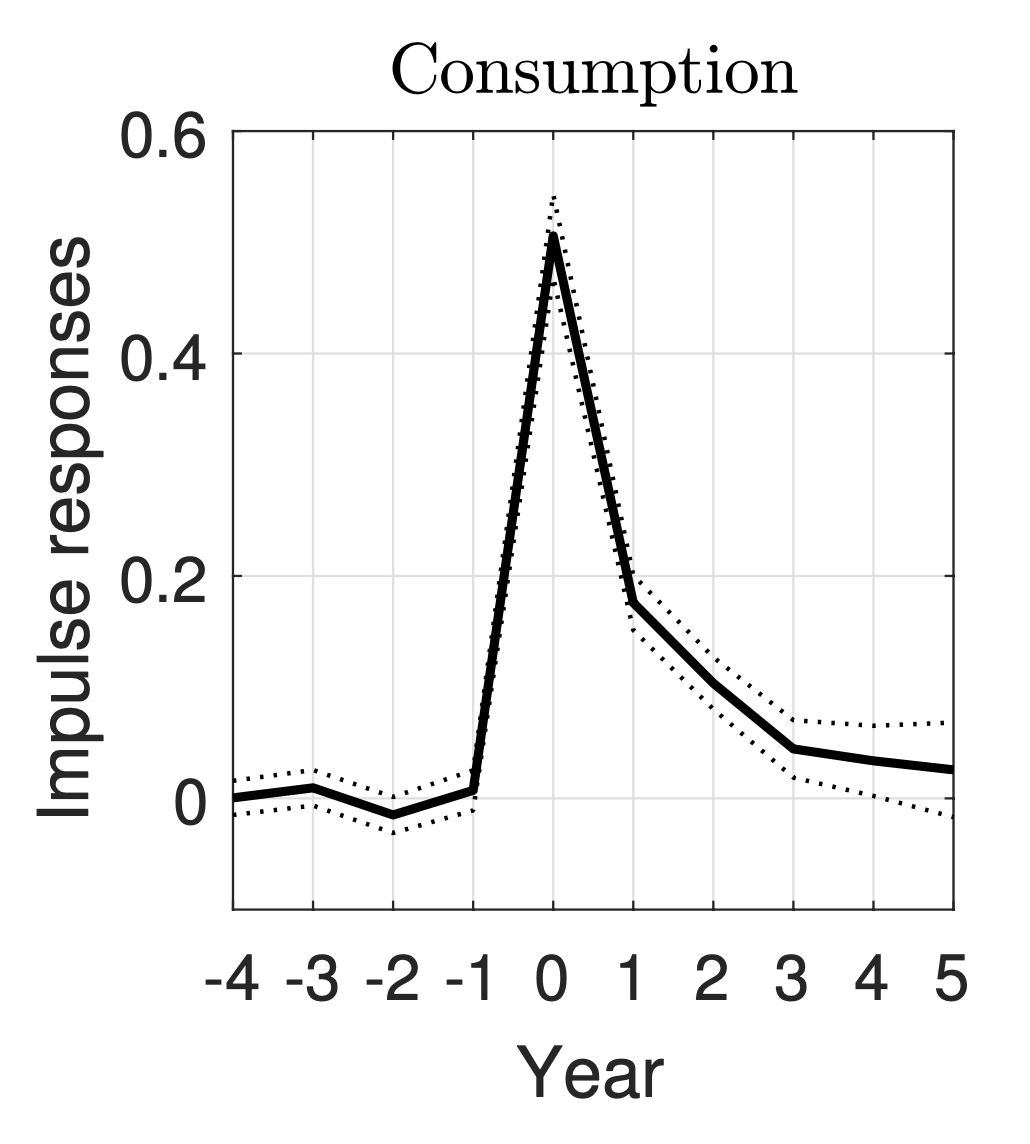
\includegraphics[scale=0.35]{figures/LotteryMPCestimate.png}}
     &  \parbox{0.4\textwidth}{
     		
            \begin{itemize}
                \item Provides estimate of first column of $\nabla_{\bm{Y}}\pmb{\mathbb{C}}$. 
                \item Need a model to extrapolate. 
%                \item Key 
            \end{itemize} Source: Fagereng, Holm, Natvik (2018) } 
%            \\
%             & 
%    $\bullet$  \\
 %    \begin{itemize}
%        \item Provides estimate of first column.
%        \item Need a model to extrapolate.
%    \end{itemize}
    \end{tabular}
\end{frame}


\begin{frame}
    \frametitle{iMPCs in the Models}
    \centering
    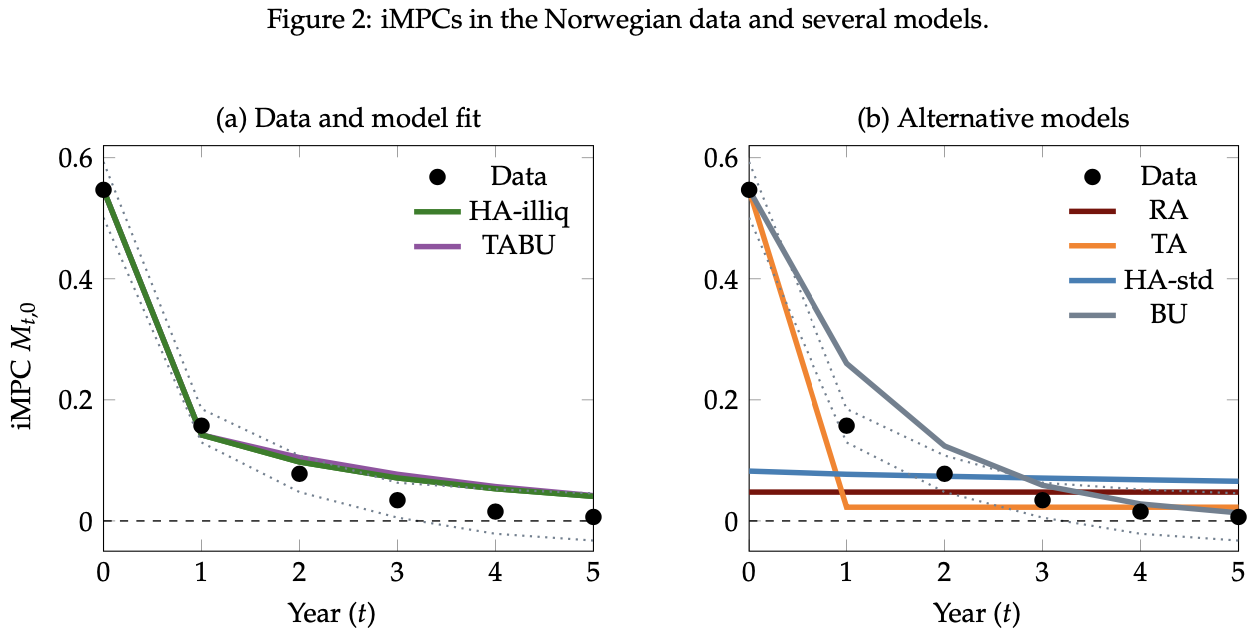
\includegraphics[scale=0.5]{figures/ARSFIG2.png}
\end{frame}

%\begin{frame}
%    \frametitle{Bonus: Durables}
%    Own figure
%\end{frame}

\begin{frame}
    \frametitle{Model Extrapolation}
    \centering
    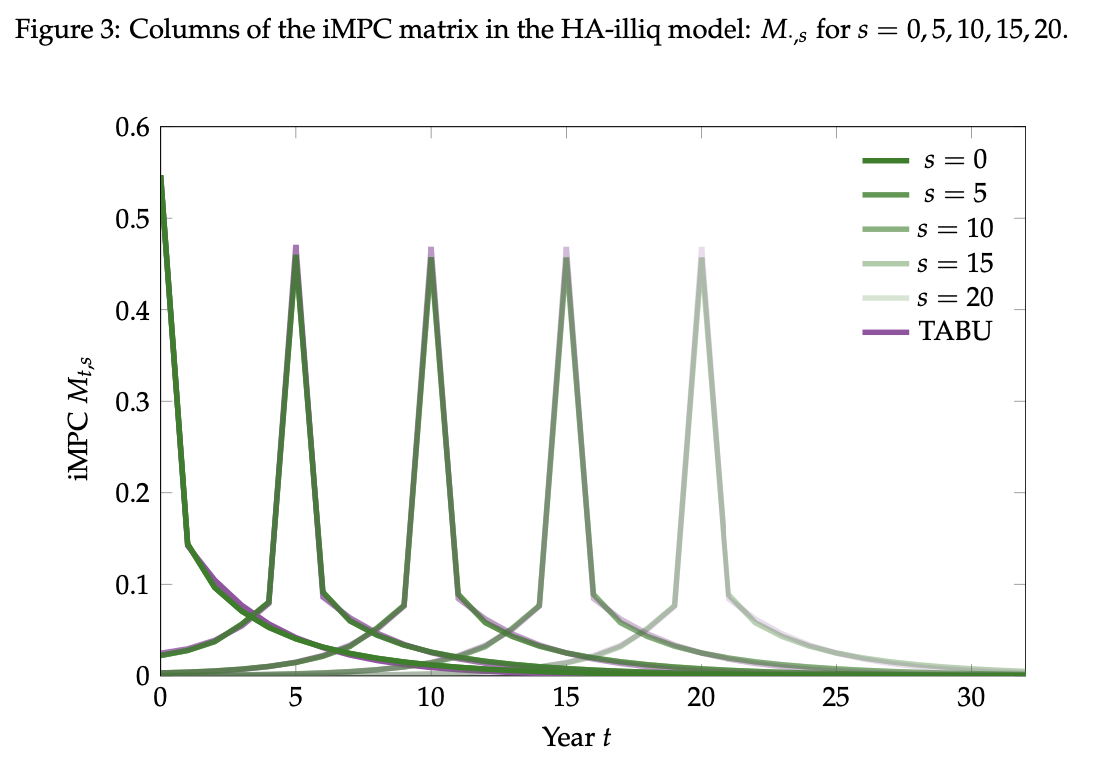
\includegraphics[scale=0.5]{figures/ARSFIG3.png}
\end{frame}


\begin{frame}
    \frametitle{Fiscal Policies: All Models}
    \centering
    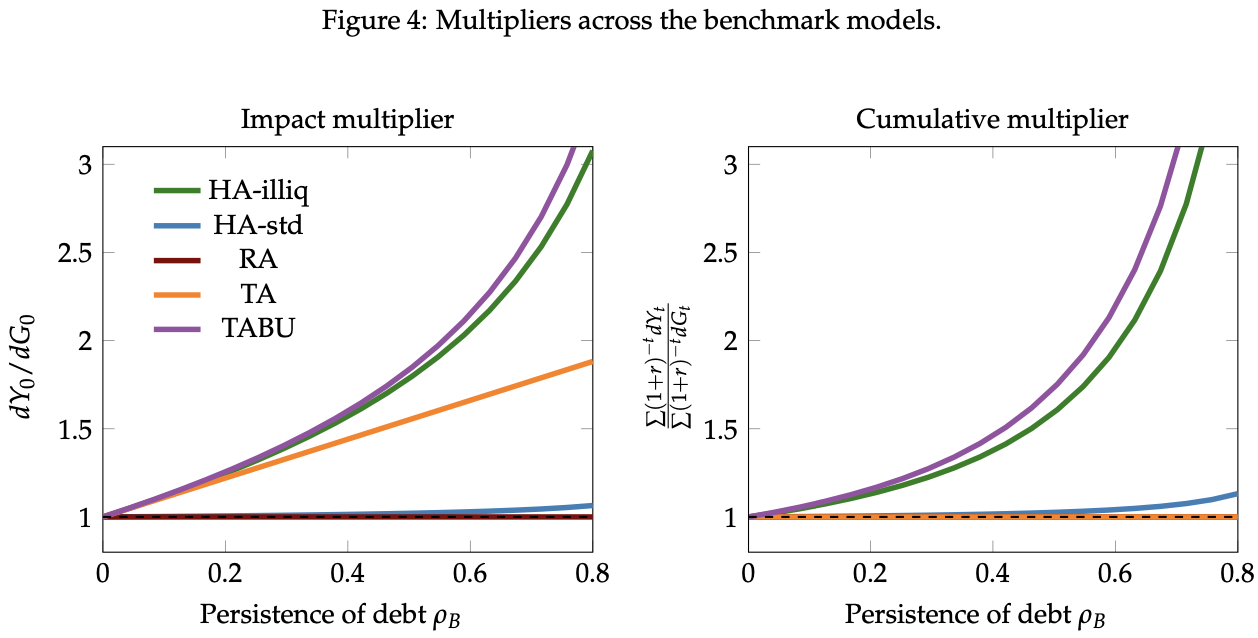
\includegraphics[scale=0.5]{figures/ARSFIG4.png}
\end{frame}

%\begin{frame}
%    \frametitle{Bonus: Regional Estimates?}
%    Own figure
%\end{frame}


\begin{frame}
    \frametitle{Quantitative Model}
    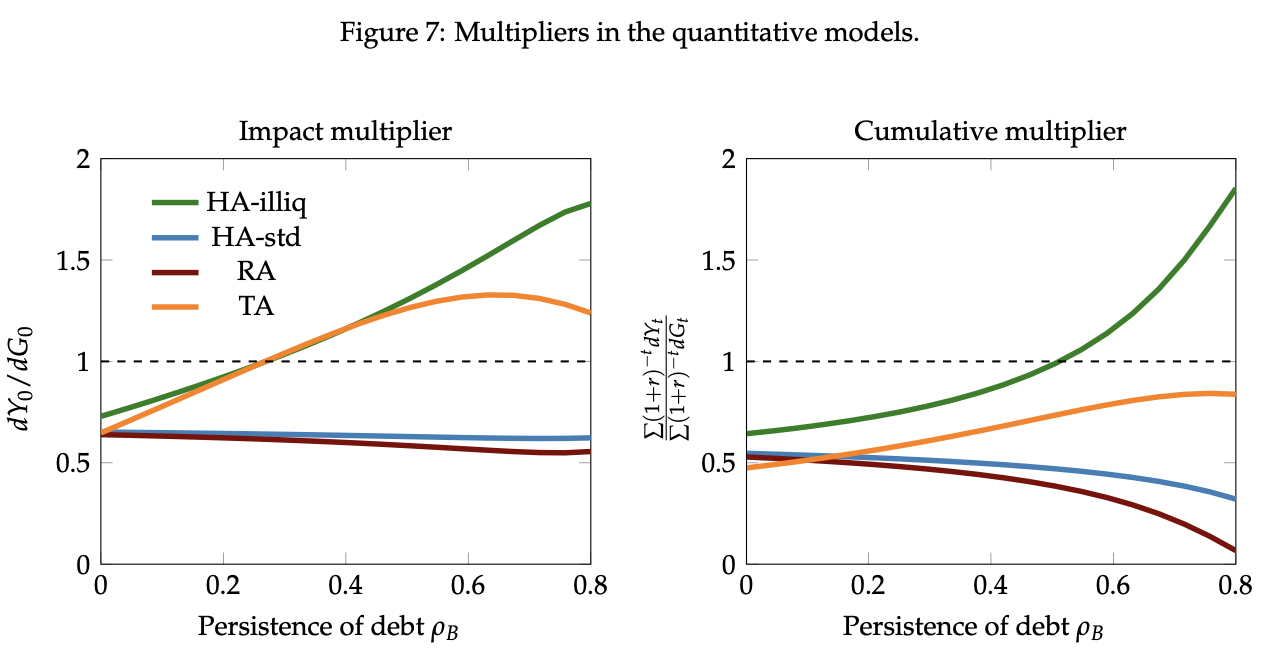
\includegraphics[scale=0.5]{figures/ARSFIG7.png}
    \begin{itemize}
    	\item What does this tell us about supply elasticities?
    \end{itemize}
\end{frame}

\begin{frame}
    \frametitle{Private Deficits}
    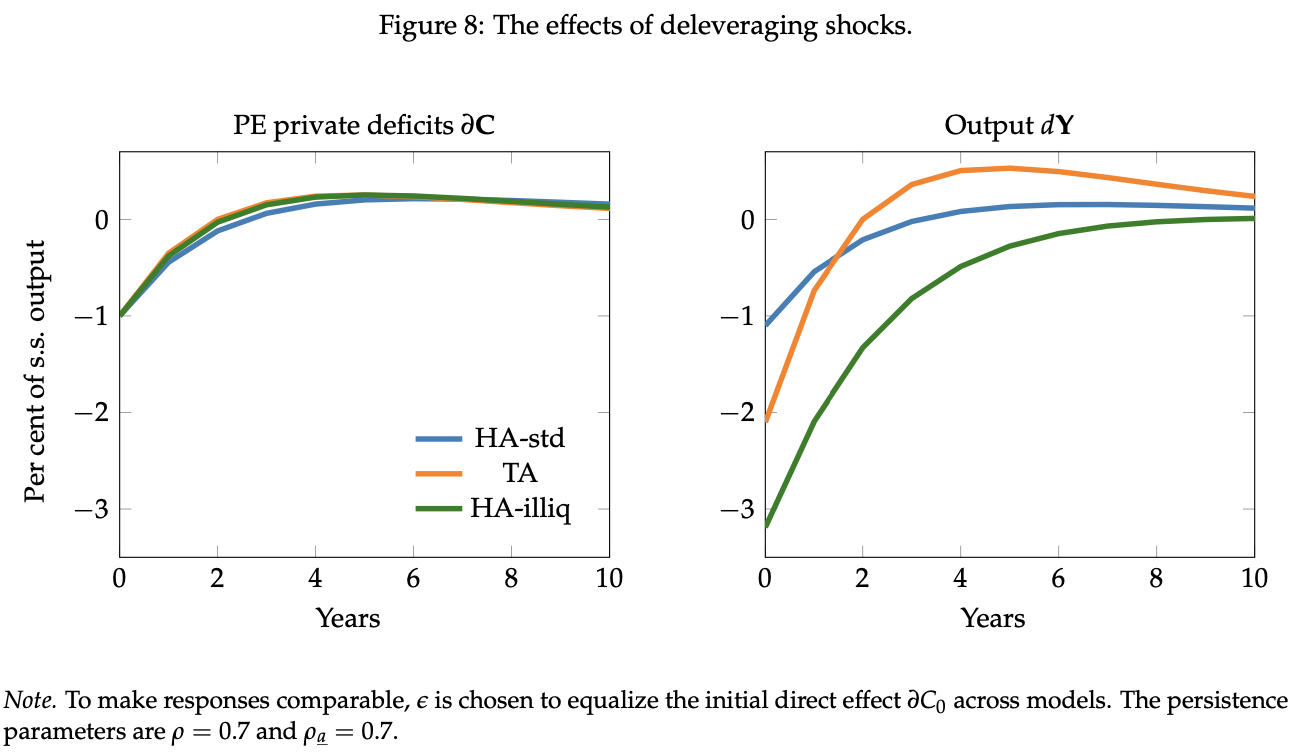
\includegraphics[scale=0.5]{figures/ARSFIG8.png}
    \begin{itemize}
    	\item Why so much amplification?
    \end{itemize}
\end{frame}

%%%%%%%%%%%%%%%%%%%%%%%%%%%%%%%%%%%%%%%%%%%%%%%%%%
\section{Auclertn Bardoczy, Rognlie, Straub (2021)}
%%%%%%%%%%%%%%%%%%%%%%%%%%%%%%%%%%%%%%%%%%%%%%%%%%

\begin{frame}
    \frametitle{Sequence Space Methods}
    \begin{itemize}
    	\item Sequence Space methods mean we use linear algebra to solve models with rich heterogeneity. 
        \item But how do we get matrices like these: 
        \begin{align*}
            \nabla_{\bm{Y}}\pmb{\mathbb{C}} = 
            \begin{pmatrix}
                \frac{\partial C_{0}}{\partial Y_0} & \frac{\partial C_{0}}{\partial Y_1} & \hdots \\
                \frac{\partial C_{1}}{\partial Y_0} & \frac{\partial C_{1}}{\partial Y_1} & \hdots \\
                \frac{\partial C_{2}}{\partial Y_0} & \frac{\partial C_{2}}{\partial Y_1} & \hdots \\
                \vdots & \vdots & \ddots \\
            \end{pmatrix}
        \end{align*}
        \item Need to solve the household consumption problem: hard.
        \item This paper: efficient algorithm that exploits model structure and linearity to get the Jacobians of the model really fast!
    \end{itemize}
\end{frame}




\begin{frame}
    \frametitle{Krussel-Smith (1998) Economy}
    \begin{itemize}
        \item Preferences:
        \begin{align*}
        	V_t(e,a_{-}) = \max_{c,k} u(c) + \beta \sum_{e'} V_{t+1}(e',k)P(e,e')
        \end{align*}
        \item Budget constraint
        \begin{align*}
        	c+k = (1+r_t)k_{-}+w_t e n
        \end{align*}
        \item Borrowing constraint
        \begin{align*}
        	k \ge 0
        \end{align*}
        \item Optimal policy:
        \begin{align*}
        	c_t^*(e,k_{-}),\; k_t^*(e,k_{-})
        \end{align*}
        \item Functions of $\{r_t,w_t\}_{t\ge 0 }$.
	\end{itemize}
\end{frame}

\begin{frame}
    \frametitle{Aggregating Consumer Problem}
    \begin{itemize}
        \item Distribution of capital and productivity:
        \begin{align*}
        	D_{t+1}(e',K) = \sum_e D_t(e,k_t^{*-1}(e,K))P(e,e')
        \end{align*}
        \item Given $D_0$, $D_{t+1}(e',K)$ are also functions of $\{r_t,w_t\}_{t\ge 0 }$.
        \item Aggregate capital holdings are therefore also a function of $\{r_t,w_t\}_{t\ge 0 }$.:
        \begin{align*}
        	\mathcal{K}_t(\{r_s,w_s\}_{s\ge 0 }) = \sum_e \int_{k_{-}} k_t^*(e,k_{-}) D_t(e,dk_{-})
        \end{align*}
        \item The function $\mathcal{K}_t$ maps an aggregate sequence $\{r_t,w_t\}_{t\ge 0 }$ into another aggregate sequence $\{K_t\}_{t\ge 0}$.
        \item The dimensionality of this problem is the length of the sequence $T$.
	\end{itemize}
\end{frame}


\begin{frame}
    \frametitle{Firm and Market Clearing}
    \begin{itemize}
        \item Keep this simple:
        \begin{align*}
        	Y_t &= Z_t K_{t-1}^{\alpha} N_t^{1-\alpha} \\
        	 r_t &= \alpha  Z_t K_{t-1}^{\alpha-1} N_t^{1-\alpha} - \delta \\
        	 w_t &= (1-\alpha) Z_t K_{t-1}^{\alpha} N_t^{-\alpha}
        \end{align*}
        \item Labor supply fixed in this problem so
        \begin{align*}
        	N_t = \sum \pi(e) en
        \end{align*}
        \item Market for capital has to clear
        \begin{align*}
        	&H_t(\bm{K},\bm{Z})  \\
        	&\equiv \mathcal{K}_t\left(\left\{\alpha  Z_s \left(\frac{K_{s-1}}{\sum \pi(e) en}\right)^{\alpha-1} - \delta,(1-\alpha) Z_s \left(\frac{K_{s-1}}{\sum \pi(e) en}\right)^{\alpha}\right\}_{s\ge 0 } \right)\\
        	&\qquad  - K_t = 0
        \end{align*}
	\end{itemize}
\end{frame}

\begin{frame}
    \frametitle{IRFs}
    \begin{itemize}
        \item Why is this useful? From implicit function theorem,
        \begin{align*}
        	d\bm{K} = - \bm{H_{K}}^{-1}\bm{H_Z} d\bm{Z}
        \end{align*}
        \item[$\Rightarrow$] To get IRFs need only the Jacobians of the market clearing condition w.r.t. the sequences $\bm{H_{K}},\bm{H_Z}$.
        \item How do we get these Jacboians? From the chain rule:
        \begin{align*}
        	[\bm{H_{K}}]_{t,s} = \frac{\partial \mathcal{K}_t}{\partial r_{s+1}}\frac{\partial r_{s+1}}{\partial K_s} + \frac{\partial \mathcal{K}_t}{\partial w_{s+1}}\frac{\partial w_{s+1}}{\partial K_s} - 1_{\{s=t\}}
        \end{align*}
        \item Some of these derivatives we can calculate analytically: $\frac{\partial r_{s+1}}{\partial K_s}, \frac{\partial w_{s+1}}{\partial K_s}, \frac{\partial r_{s}}{\partial Z_s}, \frac{\partial w_{s}}{\partial Z_s}$. 
        \item Others we have to compute numerically.
	\end{itemize}
\end{frame}


\begin{frame}
    \frametitle{General IRFs from One-Time Computation}
    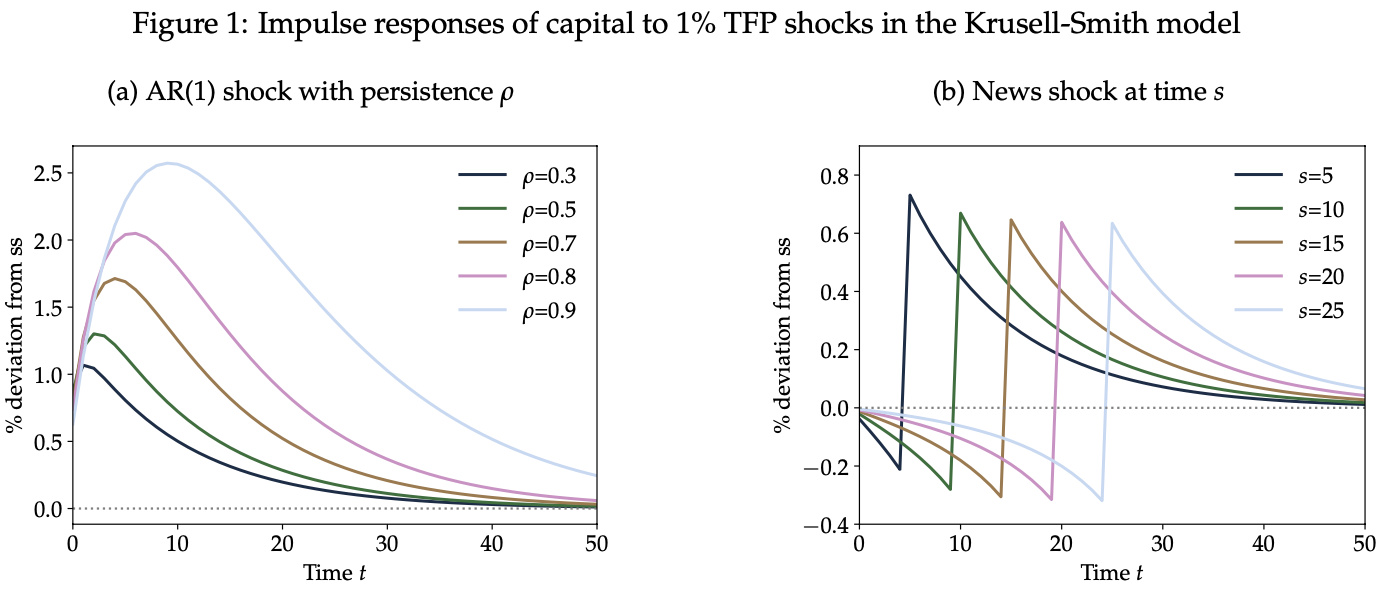
\includegraphics[scale=0.5]{figures/ABRSFIG1.png}
\end{frame}

\begin{frame}
    \frametitle{Fake News Algorithm}
    \begin{itemize}
        \item Goal: efficient computation of Jacobians.
        \item Framework:
        \begin{align*}
        	\bm{v}_t &= v(\bm{v}_{t+1},\bm{X}_t) \\
        	\bm{D}_{t+1} &= \Lambda(\bm{v}_{t+1},\bm{X}_t)'\bm{D}_{t} \\
        	\bm{Y}_{t} &= y(\bm{v}_{t+1},\bm{X}_t)'\bm{D}_{t} 
        \end{align*}
        \begin{itemize}
        	\item $\bm{X}_t$ are inputs (e.g., $Z_t$).
        	\item $\bm{Y}_t$ are outputs (e.g., $C_t, K_t$).
        	\item $\bm{D}_t$ is the discretized distribution.
        \end{itemize}
        \item In sequence space:
        \begin{align*}
        	\bm{Y} = h(\bm{X})
        \end{align*}
        \item Want: $\mathcal{J} = \pmb\nabla h_{\bm{Y}}(\bm{X}^{SS})$
      \end{itemize}
\end{frame}

\begin{frame}
    \frametitle{Brute Force}
    \begin{itemize}
    	\item Column $s$ of $\mathcal{J}_X^Y$ is IRF of outcome (e.g., capital) to a one-time shock (e.g. productivity) at $s$, $\bm{X}^s = \bm{X}_{ss} + \bm{e}^s dx \equiv \bm{X}_{ss} + d \bm{X}^s$. 
        \item Solve problem backward given the known sequence of $\bm{X}$ to get value functions $\bm{v}_{t}$, policy functions $\bm{y}_t^s$, and transition matrices $\Lambda(\bm{v}_{t+1},\bm{X}_t)'$.
        \item Given optimal policy functions iterate distribution of agents forward starting from steady state,
        \begin{align*}
    		\bm{D}_{t+1}^s &= (\Lambda_t^s) \bm{D}_t^s 
    	\end{align*}
        \item Aggregate policy functions using the distribution to get outcome
        \begin{align*}
    		\mathcal{Y}_t^s &= (\bm{y}_t^s)'\bm{D}_t^s 
    	\end{align*}
        \item Repeat for $s=0,...,T$ to get all columns of $\mathcal{J}$.
%        \item Repeat for all other aggregate sequences (e.g., $r_t$).
        \item This ``brute force'' method works but is very slow.
    \end{itemize}
\end{frame}


\begin{frame}
    \frametitle{Algorithm: Efficient backward step}
    \begin{itemize}
    	\item Lemma 1: for any $s\ge 1$, $t\ge 1$:
    	\begin{align*}
    		\bm{y}_t^s = \begin{cases}
    			\bm{y}_{ss} & s<t \\
    			\bm{y}_{T-1-(s-t)}^{T-1} & s \ge t
    		\end{cases},\qquad  \Lambda_t^s = \begin{cases}
    			 \Lambda_{ss} & s<t \\
    			 \Lambda_{T-1-(s-t)}^{T-1} & s \ge t
    		\end{cases}
    	\end{align*}
    	\item Policy functions at $t$ for shock at $t+s$ the same as policy function at $0$ for shock at $s$. 
        \item[$\Rightarrow$] Policy functions need to be solved backwards only once starting with a shock at $T-1$.
%        
        \item For any time after the shock, the policy functions are the same as in steady state.
        \item Key: policy function cannot directly depend on distribution of agents
      \end{itemize}
\end{frame}

\begin{frame}
    \frametitle{Fake News}
    \begin{itemize}
    	\item Denote the sequence $\bm{\epsilon}^s$ in which $\epsilon_s=1$ and zero otherwise:
        \begin{align*}
    		\epsilon_t = \begin{cases}
    			1 & t=s \\
    			0 & t\ge0, t\neq s
    		\end{cases}
    	\end{align*}
        \item Let $\eta_t^s$ be a fake news shock for $\epsilon_t$:
        \begin{itemize}
        	\item At $t$ learn that $\epsilon_{s}=1$ with certainty.
        	\item At $t+1$ lean that $\epsilon_{s}=0$.
        	\item $\E_{k}\eta_t^s=0$ for all $k<t$.
        \end{itemize}
        \item Lemma: The sequence $\bm{v}^s$
        \begin{align*}
    		\nu_t = \begin{cases}
    			\eta_t^{s-t} & t<s \\
    			1 & t= s \\
    			0 & t>s
    		\end{cases}\\
    	\end{align*}
        takes on the same expected values and realized values as $\bm{\epsilon}^s$.
	\end{itemize}
\end{frame}


\begin{frame}
    \frametitle{Advantage of Fake News}
    \begin{itemize}
    	\item Given linearization only care about expected values and realized values.
    	\item Rather than compute IRFs to $\bm{\epsilon}^s$ for $s\ge 0$, we need IRFs to fake news shocks $\eta^s$ for $s\ge 0$ and contemporaneous shock $\bm{\epsilon}^0$.
    	\item This is more efficient because $\eta^s$ and $\bm{\epsilon}^0$ share a common feature: the policy function only changes in the period the shock becomes known and then reverts. From then on we only need to solve the distribution forward using steady state policy functions.
	\end{itemize}
\end{frame}


\begin{frame}
    \frametitle{Algorithm: Fake News}
    \begin{itemize}
%    	\item Idea: exploit how columns in the Jacobian relate to one another.
        \item Define the difference in outcomes at $t$ for shock at $s$ versus outcomes at $t-1$ for shock at $s-1$.
        \begin{align*}
        	\mathcal{F}_{t,s}dx \equiv d\mathcal{Y}_{t}^{s} - d\mathcal{Y}_{t-1}^{s-1}
        \end{align*}
        \item Not zero: policy function the same, but distribution different.
        \item Lemma:
        \begin{align*}
        	\mathcal{F}_{t,s}dx = \bm{y}_{ss}' (\Lambda_{ss}')^{t-1}d\bm{D}_1^s
        \end{align*}
        \item Policy functions the same. The only difference is the initial distribution.
        \item To a first order, the distribution affects outcomes as if all agents followed their steady state policy functions.
	\end{itemize}
\end{frame}

\begin{frame}
    \frametitle{Fake News Interpretation}
     \begin{align*}
        	\mathcal{F}_{t,s}dx = \bm{y}_{ss}' (\Lambda_{ss}')^{t-1}d\bm{D}_1^s
        \end{align*}
    \begin{itemize}
        \item Agents at $t=0$ were told a shock will happen at $t=s$.
        \item They change their optimal policy rules resulting in a new distribution of outcomes at $t=1$, $d\bm{D}_1^s$.
        \item At $t=1$ agents learn (to their surprise) that the shock does not happen.
        \item So all policy rules revert to steady state.
        \item But the distribution has not reverted to steady state and will affect economic outcomes.
        \item $\bm{y}_{ss}' (\Lambda_{ss}')^{t-1}d\bm{D}_1^s$ traces out IRF from $t=1$ onwards to a first order.
        \item Requires only one updating step in solving $d\bm{D}_1^s$
	\end{itemize}
\end{frame}


\begin{frame}
    \frametitle{Fake News Matrix}
    \begin{itemize}
    	\item Define the fake news matrix as
    	\begin{align*}
    		\mathcal{F}_{t,s}dx \equiv \begin{cases}
    			d\mathcal{Y}_0^s & t=0 \\
    			\bm{y}_{ss}' (\Lambda_{ss}')^{t-1}d\bm{D}_1^s & t\ge 1
    		\end{cases}
    	\end{align*}
        \item Then the Jacobian of $h$ is given by
        \begin{align*}
        	\mathcal{J}_{t,s} = \sum_{k=0}^{\min\{s,t\}}\mathcal{F}_{t-k,s-k}
        \end{align*}
        \item $t=0$ follows by definition.
        \item Why does this make sense?
	\end{itemize}
\end{frame}


\begin{frame}
    \frametitle{Fake News Matrix Examples}
    \begin{itemize}
        \item $t>0,s=0$:
        \begin{align*}
        	\mathcal{J}_{t,0} = \bm{y}_{ss}'(\Lambda_{ss}')^{t-1} d\bm{D}_1^0
        \end{align*}
        \begin{itemize}
        	\item Shock at $0$ affected distribution at $1$. Now trace out this effect.
        \end{itemize}
       	\item $t=1,s=1$:
        \begin{align*}
        	\mathcal{J}_{1,1} = d\mathcal{Y}_0^0 + \bm{y}_{ss}' d\bm{D}_1^1
        \end{align*}
        \begin{itemize}
        	\item Sum of surprise contemporaneous shock and fake news shock.
        \end{itemize}
        \item $t=1,s=2$:
        \begin{align*}
        	\mathcal{J}_{1,2} = d\mathcal{Y}_0^1 + \bm{y}_{ss}' d\bm{D}_1^2
        \end{align*}
        \begin{itemize}
        	\item As if we got news today about shock tomorrow, but taking into account change in distribution given that news was known earlier.
        \end{itemize}
        \begin{align*}
        	\mathcal{J}_{3,4} = d\mathcal{Y}_0^1 + \bm{y}_{ss}'  d\bm{D}_1^2 + \bm{y}_{ss}' (\Lambda_{ss}') d\bm{D}_1^3 + \bm{y}_{ss}' (\Lambda_{ss}')^{2} d\bm{D}_1^4
        \end{align*}
	\end{itemize}
\end{frame}

\begin{frame}
    \frametitle{Bottom Line}
    \begin{itemize}
        \item $t=1,s=0$:
        \begin{align*}
        	\mathcal{J}_{t,s} = \mathcal{J}_{t-1,s-1} + \mathcal{F}_{t,s} 
        \end{align*}
        \begin{itemize}
        	\item A shock at $s$ from time $t$ looks very similar to a shock at $s-1$ from time $t-1$. 
        	\item Policy functions are exactly the same.
        	\item Only difference is that the distribution at $t$ is different from $t-1$, which is captured by the fake news term. 
        \end{itemize}
       	\item The objects we need to calculate this are:
       	\begin{enumerate}
       		\item Solve consumer problem backwards once for $T$ periods to get policy functions $\{\bm{y}^{T-1}_{T-1-s},\bm{\Lambda}^{T-1}_{T-1-s}\}_{s=0}^{T-1}$.
       		\item Get $\{d\mathcal{Y}_0^s\}_{s=0}^T$ by combining policy functions for $s=0,...,T$ with steady state distribution.
       		\item Compute $d\bm{D}_1^s$ using steady state distribution and $s=0,...,T$ policy functions.
       	\end{enumerate}
       	\item[$\Rightarrow$] Very small number of steps / computations to get all of the Jacobian and therefore the IRFs.
	\end{itemize}
\end{frame}


\begin{frame}
    \frametitle{Result}
    \centering
    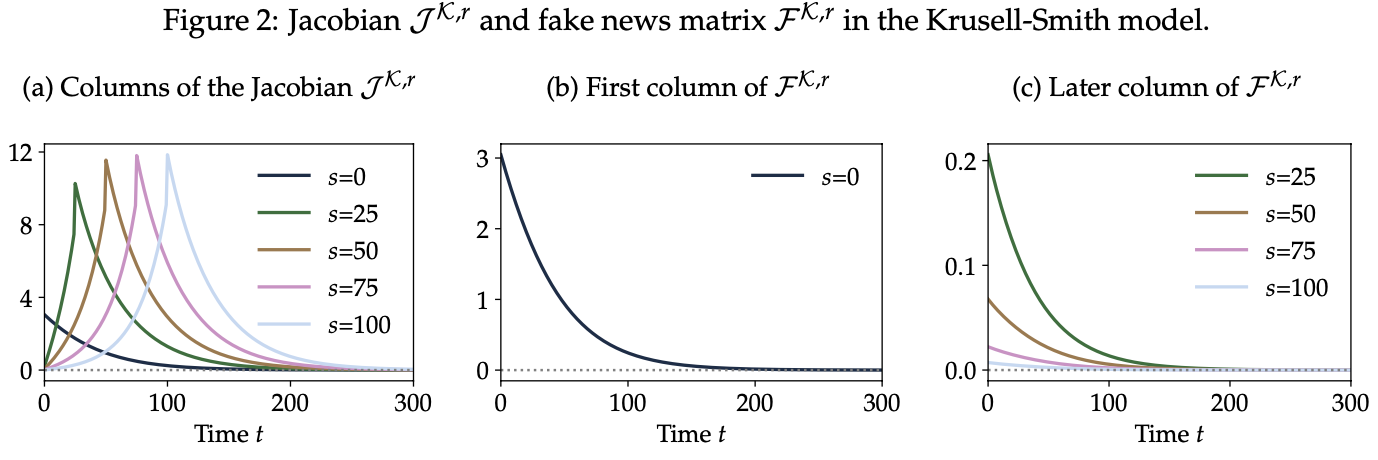
\includegraphics[scale=0.5]{figures/ABRSFIG2.png}
\end{frame}



\begin{frame}
    \frametitle{Dimensionality Reduction}
    \begin{itemize}
    	\item The dimensionality of the problem is $T \times \text{number of variables}$, but with large $T$ and many variables this can get complicated.
    	\item Solution: substitute out for some variables, like we did for $r_t,w_t$ earlier. 
    	\item This can be automated by writing the model in separate blocks.
    	\item E.g., firm block $r_t = \alpha  Z_t K_{t-1}^{\alpha-1} N_t^{1-\alpha} - \delta $ and $ w_t = (1-\alpha) Z_t K_{t-1}^{\alpha} N_t^{-\alpha}$ can be used to solved out for $r_t,w_t$ as a function of $Z_t,K_t,N_t$.
    	\item Each block takes inputs (e.g., $Z_t,K_t,N_t$) and computes outputs ($r_t,w_t$).
	\end{itemize}
\end{frame}

\begin{frame}
    \frametitle{Directed Acyclical Graph}
    \begin{center}
    	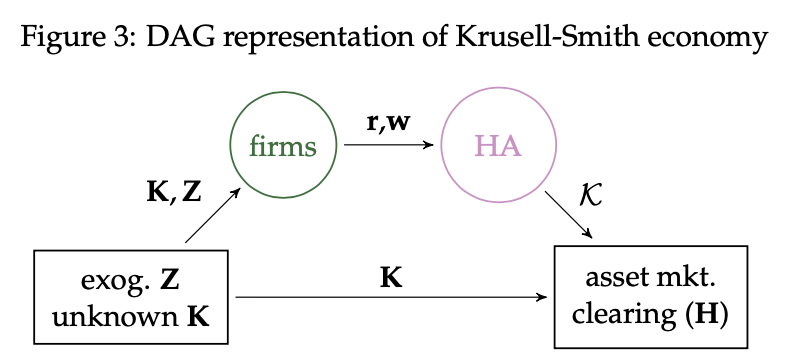
\includegraphics[scale=0.5]{figures/ABRSFIG3.png}
    \end{center}
    \begin{itemize}
    	\item The computer can do the substitution if we write the model as a Directed Acyclical Graph (DAG).
    	\item Dimensionality $T \times 2$ even though we have 4 endogenous variables.
    	\item Restriction: cannot have cycle. E.g., if $K$ was not an unknown, the graph would be cylical.
        \item Always(?) possible to write model as DAG.
%        \item Computer does the sorting and substituting out.
	\end{itemize}
\end{frame}


\begin{frame}
    \frametitle{More}
    \begin{itemize}
    	\item How to pick $T$: check if higher $T$ matters for IRFs. Authors recommend $T=300-1000$.
    	\item Estimation:  Can compute moments and likelihood quickly from Jacobians. Limit is how quickly you can recompute Jacobians given new parameter values.   	
    	\item Non-linear perfect foresight dynamics.
	\end{itemize}
\end{frame}

\begin{frame}
    \frametitle{More}
    \begin{center}
    	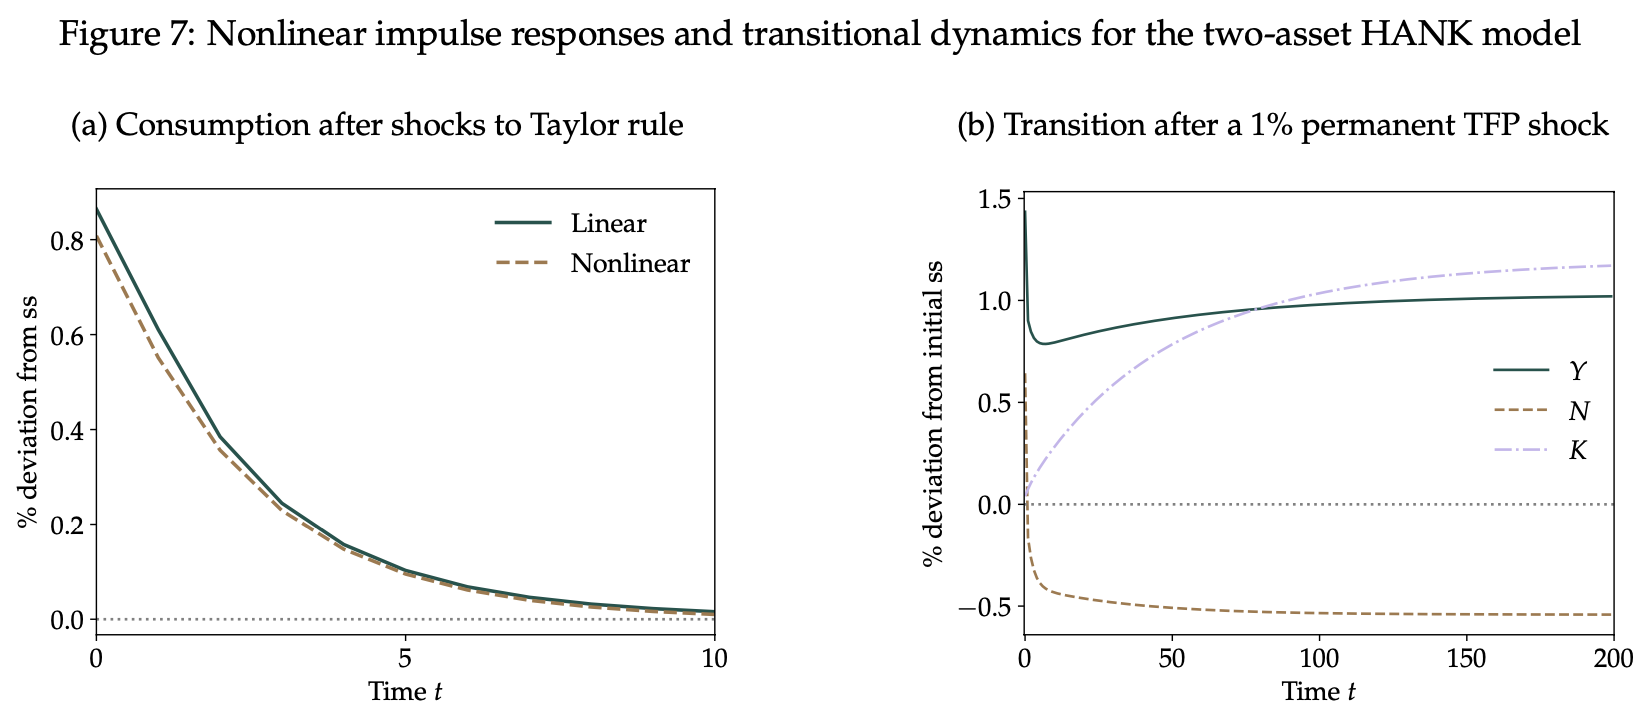
\includegraphics[scale=0.4]{figures/ABRSFIG7.png}
    \end{center}
    \begin{itemize}
    	\item See also McKay and Wieland (2022, Econometrica) for how to implement a ZLB.
    \end{itemize}
\end{frame}



\end{document}